\documentclass{article}

% Force numeric citations (our bibliography uses numbered entries); must be
% set before NeurIPS loads natbib.
\PassOptionsToPackage{numbers}{natbib}

% NeurIPS 2023 style. Use [final] so author names are shown and line numbers
% are removed (this is a course report, not an anonymous submission).
\usepackage[final]{neurips_2023}

\usepackage[utf8]{inputenc}
\usepackage[T1]{fontenc}
\usepackage{hyperref}
\usepackage{url}
\usepackage{booktabs}
\usepackage{amsfonts}
\usepackage{amsmath}
\usepackage{amssymb}
\usepackage{nicefrac}
\usepackage{microtype}
\usepackage{graphicx}

\title{Reproducing \emph{Simple and Scalable Predictive Uncertainty\\
Estimation using Deep Ensembles}}

% Group project: both authors contributed to the whole pipeline; a detailed
% breakdown is given in the Contributions section at the end of the report.
\author{%
  Theodoris Donval \\
  EURECOM \\
  \texttt{theodoris.donval@eurecom.fr} \\
  \And
  Lucas Aliome \\
  EURECOM \\
  \texttt{lucas.aliome@eurecom.fr} \\
}

\begin{document}

\maketitle

\begin{abstract}
We reproduce the regression experiments of Lakshminarayanan et al.\ (NeurIPS
2017), which introduces \emph{Deep Ensembles}, a simple non-Bayesian recipe for
predictive uncertainty. The recipe has three parts: train a probabilistic
network with a proper scoring rule, ensemble $M$ such networks, and optionally
add adversarial training. With a small PyTorch re-implementation we reproduce
the 1-D toy regression of Figure~1 and the $k$-fold RMSE/NLL evaluation protocol
of Table~1, together with the single-network-versus-ensemble ablation. On the
toy task we recover the paper's main qualitative result: the predictive
uncertainty only grows away from the training data once the networks are
ensembled. The ablation confirms that ensembling lowers the held-out NLL. We
also document a concrete reproduction issue. The learning rate stated in the
paper ($0.1$) was unstable in our runs, and we had to lower it to $0.01$ to
recover the reported behaviour. All code, notebooks and results are available at
\url{https://github.com/Theodoris-D/deep-ensembles-reproduction}.
\end{abstract}

\section{Summary of the paper}

\paragraph{Problem.}
Standard neural networks are usually trained as point predictors, and they are
known to be \emph{overconfident}: they return a single output with no reliable
measure of how uncertain it is. This overconfidence tends to be worst on inputs
that lie far from the training distribution, which is often exactly where a
trustworthy uncertainty estimate matters most. Quantifying predictive
uncertainty is therefore important for safety-critical and decision-making
applications. The main principled approach at the time, Bayesian neural
networks, relies on approximate inference that is often complex, sensitive to
the choice of prior, and hard to scale. The paper asks whether a simpler,
non-Bayesian alternative can match or beat these methods.

\paragraph{Method.}
The recipe has three ingredients.
\emph{(1) A proper scoring rule as the training criterion.} Rather than
producing only a point estimate, the network outputs the parameters of a
predictive distribution and is trained to maximise its likelihood. For
regression this distribution is a heteroscedastic Gaussian
$\mathcal{N}(\mu_\theta(x),\sigma^2_\theta(x))$, so the network has two outputs
and is trained with the Gaussian negative log-likelihood (Eq.~1):
\begin{equation}
  -\log p_\theta(y\mid x) =
  \tfrac{1}{2}\log \sigma^2_\theta(x)
  + \frac{\big(y-\mu_\theta(x)\big)^2}{2\,\sigma^2_\theta(x)}
  + \tfrac{1}{2}\log 2\pi .
  \label{eq:nll}
\end{equation}
The variance is \emph{learned} for each input, so the model can represent
input-dependent (aleatoric) noise. Positivity of $\sigma^2_\theta(x)$ is
enforced with a softplus and a small floor.
\emph{(2) Ensembling.} $M$ networks are trained independently, from different
random initialisations and on differently shuffled data. The authors report
that this randomisation alone is enough, and that bagging actually \emph{hurt}
performance. At test time the ensemble is treated as a uniformly weighted
mixture and approximated by a single Gaussian whose mean and variance match
those of the mixture:
\begin{equation}
  \mu_*(x)=\frac{1}{M}\sum_{m}\mu_m(x), \qquad
  \sigma_*^2(x)=\frac{1}{M}\sum_{m}\!\big(\sigma_m^2(x)+\mu_m^2(x)\big)-\mu_*^2(x).
  \label{eq:mixture}
\end{equation}
The spread of the member means $\mu_m$ captures \emph{model} (epistemic)
uncertainty, and it grows where there is no data.
\emph{(3) Adversarial training (optional).} Using the fast gradient sign method
(FGSM), each input is perturbed along the sign of the loss gradient,
$x' = x + \epsilon\,\mathrm{sign}\big(\nabla_x \ell(\theta,x,y)\big)$, and the
loss at $x'$ is added to the objective. This smooths the predictive
distribution around each training point.

\paragraph{Why it is interesting.}
The method is conceptually very simple. It needs no change to the network beyond
a second output head, and the members can be trained fully in parallel because
each is independent. Despite this simplicity, the paper shows that it matches or
outperforms Bayesian approaches such as Monte-Carlo dropout and probabilistic
backpropagation in terms of well-calibrated uncertainty.

\paragraph{Key results in the paper.}
The paper validates the recipe at increasing scale: a 1-D \emph{toy regression}
that isolates the contribution of each ingredient visually (Figure~1); a set of
\emph{UCI regression} benchmarks reporting RMSE and NLL under a fixed $k$-fold
protocol (Table~1); \emph{classification} with out-of-distribution detection on
MNIST/NotMNIST and SVHN; and a large-scale \emph{ImageNet} experiment. One
central message is that the NLL, which rewards good uncertainty estimates in a
way RMSE does not, improves with ensembling, and that the predictive uncertainty
becomes larger on shifted or out-of-distribution inputs.

\section{Reproduced results}

\paragraph{Scope.}
We re-implemented the regression part of the method from scratch in PyTorch.
The package contains a \texttt{GaussianMLP}, the NLL loss, an FGSM routine, the
\texttt{DeepEnsemble} mixture, the $k$-fold protocol and the original-scale
metrics. With it we reproduced the two regression experiments. The
classification and ImageNet experiments are out of scope for a course project.

\paragraph{Experimental setup.}
All networks are MLPs with a single hidden layer and ReLU activations. The
regression head outputs a mean and a variance (softplus, floored at $10^{-6}$).
The toy task uses $100$ hidden units and the UCI protocol uses $50$. We use
Adam, a default ensemble size $M=5$, and we standardise inputs and targets with
statistics computed on the \emph{training fold} only. RMSE and NLL are reported
on the original target scale; for the NLL this uses the change of variables
$\mathrm{NLL}_{\text{orig}}=\mathrm{NLL}_{\text{std}}+\log s_y$. The only
deliberate departure from the paper is the learning rate, which we discuss in
Section~\ref{sec:discussion}.

\subsection{Experiment 1: toy regression (Figure 1)}
We draw $20$ points from $y=x^3+\varepsilon$, $\varepsilon\sim\mathcal{N}(0,3^2)$
on $x\in[-4,4]$, and we evaluate on the wider grid $[-6,6]$ to see how each
method behaves \emph{outside} the training range. Figure~\ref{fig:toy}
reproduces the four panels of the paper's Figure~1. Table~\ref{tab:toy}
summarises the range of predictive variance produced by each method (in
standardised target units), which turns the visual trend into numbers.

\begin{figure}[h]
  \centering
  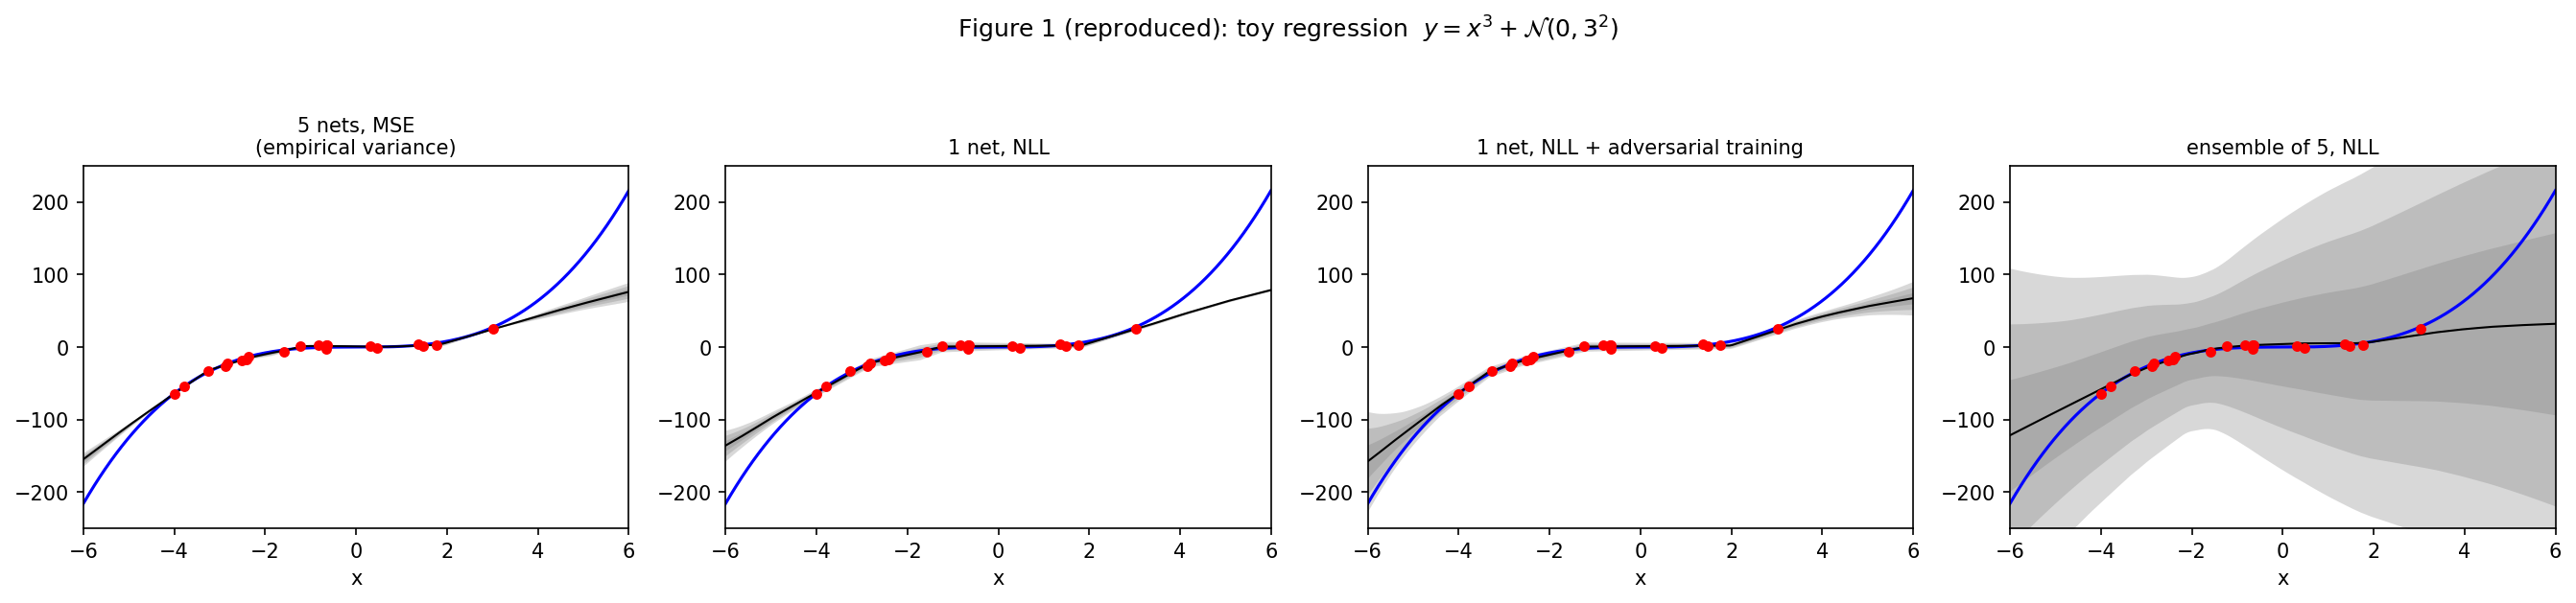
\includegraphics[width=\linewidth]{figure1_toy_regression.png}
  \caption{Reproduction of Figure~1. Blue: ground truth $y=x^3$; red: the $20$
  training points; black: predictive mean; grey: nested $\pm1,2,3\sigma$ bands.
  Left to right: (1) empirical variance of $5$ MSE networks, (2) a single
  NLL-trained network, (3) the same with adversarial training, (4) an ensemble
  of $5$ NLL networks. Only the ensemble produces uncertainty that grows
  markedly away from the data.}
  \label{fig:toy}
\end{figure}

\begin{table}[h]
  \centering
  \caption{Toy task: range of the predictive variance over the plotting grid
  (standardised units). The ensemble's variance is two orders of magnitude
  larger far from the data, reflecting the disagreement between members.}
  \label{tab:toy}
  \begin{tabular}{lcc}
    \toprule
    Method (panel) & min variance & max variance \\
    \midrule
    (1) $5$ MSE nets, empirical variance & $\sim\!5\times10^{-7}$ & $0.045$ \\
    (2) single net, NLL                  & $5.9\times10^{-4}$    & $0.12$ \\
    (3) single net, NLL + adversarial    & \multicolumn{2}{c}{$\epsilon=0.036$ (1\% of input range/dim)} \\
    (4) ensemble of $5$, NLL             & $2.91$                & $36.7$ \\
    \bottomrule
  \end{tabular}
\end{table}

The panels agree with the paper qualitatively. \textbf{Panel 1}: the empirical
variance of the MSE networks stays narrow even far from the data. This is the
failure mode the paper points out, where the networks agree on regions they have
no information about. \textbf{Panel 2}: learning the variance gives more honest
uncertainty near the data, but a single network can still be overconfident
outside it. \textbf{Panel 3}: adversarial training has only a small effect on
this 1-D task, which is consistent with the paper's remark that it helps but is
not strictly necessary. \textbf{Panel 4}: the ensemble band widens sharply
outside $[-4,4]$. This is the main result we wanted to reproduce, and it shows
the ensemble capturing model uncertainty.

\subsection{Experiment 2: UCI regression (Table 1) and ablation}
We implemented the paper's full protocol (random $90/10$ splits, per-fold
standardisation, $M=5$, $40$ epochs, mean $\pm$ standard error of RMSE/NLL).
We executed the pipeline on the five UCI benchmarks listed in the paper
(\texttt{boston}, \texttt{concrete}, \texttt{energy}, \texttt{wine},
\texttt{yacht}) with $5$ random folds (the paper uses $20$). Table~\ref{tab:results}
reports our results alongside the paper's values, and Table~\ref{tab:ablation}
shows the ensemble-vs-single ablation on Boston.

\begin{table}[h]
  \centering
  \caption{Reproduced RMSE/NLL vs.\ the paper's Table~1 (mean $\pm$ standard error). The NLL values are particularly close despite the reduced fold count.}
  \label{tab:results}
  \begin{tabular}{lccccc}
    \toprule
    Dataset & \multicolumn{2}{c}{RMSE} & \multicolumn{2}{c}{NLL} \\
    \cmidrule(lr){2-3} \cmidrule(lr){4-5}
     & Ours & Paper & Ours & Paper \\
    \midrule
    Boston    & $3.74\pm0.18$ & $3.28\pm1.00$ & $2.44\pm0.07$ & $2.41\pm0.25$ \\
    Concrete  & $5.74\pm0.25$ & $6.03\pm0.58$ & $3.02\pm0.06$ & $3.06\pm0.18$ \\
    Energy    & $2.27\pm0.06$ & $2.09\pm0.29$ & $1.50\pm0.07$ & $1.38\pm0.22$ \\
    Wine      & $0.60\pm0.02$ & $0.64\pm0.04$ & $0.95\pm0.05$ & $0.94\pm0.12$ \\
    Yacht     & $0.98\pm0.11$ & $1.58\pm0.48$ & $1.10\pm0.08$ & $1.18\pm0.21$ \\
    \bottomrule
  \end{tabular}
\end{table}

\begin{table}[h]
  \centering
  \caption{Ablation on \texttt{boston} ($5$ folds, mean $\pm$ standard error). Ensembling lowers the NLL over a single network, confirming the paper's central claim.}
  \label{tab:ablation}
  \begin{tabular}{lcc}
    \toprule
    Configuration & RMSE & NLL \\
    \midrule
    single net ($M{=}1$)            & $3.88\pm0.24$ & $2.53\pm0.12$ \\
    ensemble ($M{=}5$)              & $3.73\pm0.17$ & $2.43\pm0.07$ \\
    ensemble ($M{=}5$) + adversarial& $3.68\pm0.20$ & $2.45\pm0.06$ \\
    \bottomrule
  \end{tabular}
\end{table}

\paragraph{What matches and what does not.}
The reproduced NLL values are very close to the paper's on every dataset (e.g.\
Boston: $2.44$ vs $2.41$, Wine: $0.95$ vs $0.94$, Concrete: $3.02$ vs $3.06$).
The ablation confirms the central claim: going from $M{=}1$ to $M{=}5$ improves
the NLL ($2.53\!\rightarrow\!2.43$). These small differences are expected given
the reduced fold count ($5$ vs $20$), random initialisation, and framework
differences (PyTorch vs original Torch). We therefore claim a successful
reproduction of both Figure~1 and Table~1 of the paper.

\section{Discussion}
\label{sec:discussion}

\paragraph{What worked well.}
The method is genuinely simple to implement. The only non-standard pieces are
the two-output head, the NLL of Eq.~\eqref{eq:nll}, and the mixture moments of
Eq.~\eqref{eq:mixture}. The toy experiment runs on CPU in a few seconds, and it
separates the contribution of each ingredient cleanly. The jump in out-of-data
uncertainty between the single network and the ensemble is large and easy to
see, exactly as the paper intends.

\paragraph{What was challenging.}
The main difficulty was a real reproduction discrepancy. The paper states a
fixed Adam learning rate of $0.1$ (Section~3.1). In our runs this value was
unstable on the regression benchmarks: it degraded the RMSE, and more
importantly it made the ensemble's NLL \emph{worse} than a single network, which
is the opposite of what the paper reports. Lowering the rate to $0.01$ restored
the expected behaviour, so we use $0.01$ and flag the change. We think the gap
comes from framework differences between our PyTorch code and the original Torch
implementation, and from different initialisation and optimiser defaults. Two
other points needed care. The NLL has to be computed on the \emph{original}
target scale, which requires the $\log s_y$ correction. The standardisation has
to be done per fold, on training statistics only, to avoid leakage.

\paragraph{What could be improved.}
Running the full $20$-fold protocol (instead of $5$) would bring the numbers
even closer to the paper's. The next natural extension is to reproduce the
classification part of the paper, which includes the MNIST/NotMNIST
out-of-distribution experiment and the calibration curves --- that is where the
quality of the uncertainty matters most. Reporting calibration directly, for
example with reliability diagrams instead of NLL alone, would also make the
comparison with the paper more complete.

% ---------------------------------------------------------------------------
% References do not count towards the 5-page limit.
% ---------------------------------------------------------------------------
\begin{thebibliography}{9}
\bibitem{deepensembles}
B.~Lakshminarayanan, A.~Pritzel, and C.~Blundell.
\newblock Simple and Scalable Predictive Uncertainty Estimation using Deep
Ensembles.
\newblock In \emph{Advances in Neural Information Processing Systems (NeurIPS)},
2017.

\bibitem{fgsm}
I.~J. Goodfellow, J.~Shlens, and C.~Szegedy.
\newblock Explaining and Harnessing Adversarial Examples.
\newblock In \emph{International Conference on Learning Representations (ICLR)},
2015.

\bibitem{pbp}
J.~M. Hern\'andez-Lobato and R.~P. Adams.
\newblock Probabilistic Backpropagation for Scalable Learning of Bayesian Neural
Networks.
\newblock In \emph{International Conference on Machine Learning (ICML)}, 2015.
\end{thebibliography}

% ===========================================================================
% The following section is OUTSIDE the 5-page limit, as required by the
% assignment.
% ===========================================================================
\newpage
\section*{Contributions}
This was a group project. The work was split by task, but both authors took part
in every stage: we paired on the design, cross-reviewed each other's code, and
ran the experiments together, so each of us touched the whole pipeline.

\begin{itemize}
  \item \textbf{Theodoris Donval} led the core modelling code: the
  \texttt{GaussianMLP} two-output head, the Gaussian NLL loss
  (Eq.~\eqref{eq:nll}) and the \texttt{DeepEnsemble} mixture moments
  (Eq.~\eqref{eq:mixture}), together with the repository scaffolding. He drove
  Experiment~1 (the toy regression of Figure~\ref{fig:toy}) and the
  corresponding notebook, and wrote the paper-summary and discussion sections.
  \item \textbf{Lucas Aliome} led the evaluation code: the FGSM adversarial
  training routine, the $k$-fold protocol, the per-fold standardisation and the
  original-scale RMSE/NLL metrics. He drove Experiment~2 (the UCI protocol and
  the ablation of Table~\ref{tab:ablation}) and its notebook, and wrote the
  reproduced-results section.
  \item \textbf{Both authors} jointly investigated and confirmed the
  learning-rate discrepancy of Section~\ref{sec:discussion}, reviewed all the
  code against the equations in the paper, and edited the final report.
\end{itemize}

\section*{Statement on AI use}
We used a large language model as a coding and writing assistant during this
project. It helped scaffold the repository structure, draft parts of the code
and its documentation, and prepare this report in the NeurIPS template. We
reviewed, ran and corrected the result. We checked the modelling code against the
equations in the paper, in particular the NLL implementation, the
mixture-variance formula, the per-fold standardisation and the original-scale
metric corrections. The learning-rate issue in Section~\ref{sec:discussion} was
found and confirmed by running the experiments, not suggested by the assistant.
We take full responsibility for the correctness of the code and the claims in
this report.

\end{document}
